\documentclass[a5paper, 12pt]{article}
\usepackage[left=2cm, right=2cm, top=2cm, bottom=2cm]{geometry}
\setlength{\parindent}{0cm}

\usepackage{amsmath}
\usepackage{graphicx}

\begin{document}
\title{Maxwell's Equations}
\author{Ankit kumar}
\date{\today}
\maketitle

\section{Ankit kumar (me20b024)}


%A few commonly used constants, to cut down on typing and increase clarity
\def\eps0{\ensuremath{\epsilon _0}}
\def\muz{\ensuremath{\mu_0}}

%Define a closed integral construct. I had some help with making this one look nice
\def\cint#1{\ensuremath{\displaystyle\underset{\substack{\text{\tiny{closed}}\\\text{\tiny{surface}}}}{\oint} \mspace{-0.1 mu} #1}}

%Define symbols for flux, just to make sure it stays consistent throughtout the paper
\def\phie{\ensuremath{\phi_E}}
\def\phib{\ensuremath{\phi_B}}

%Define the derivatives, so don't have to do all the typing every time
\def\dA{\ensuremath{\emph{d}\vec{A}}}
\def\dB{\ensuremath{\emph{d}\vec{B}}}
\def\ds{\ensuremath{\emph{d}\vec{s}}}
\def\dt{\ensuremath{\emph{dt}}}
\def\dphie{\ensuremath{\emph{d}\phie}}
\def\dphib{\ensuremath{\emph{d}\phib}}






\subsection{Maxwell's Equations}

\indent The differential forms of Maxwell's equations as found by Heaviside, while completely valid, are now considered somewhat archaic, and have been replaced by the more useful (equivalent) integral forms. Each law is named according to the person(s) who originally discovered the connections represented by the equation. Here are the four equations:
\begin{eqnarray}
\label{eq:gauss_ele}
\text{Gauss' law for electricity:}& \displaystyle \cint{\vec{E}\cdot\dA}&=\frac{Q_{enc}}{\eps0}\\
\label{eq:gauss_mag}
\text{Gauss' law for magnetism:}& \displaystyle \cint{\vec{B}\cdot\dA}&=0\\
\label{eq:faraday}
\text{Faraday's law:}& \displaystyle\oint{\vec{E}\cdot\ds}&=-\frac{\dphib}{\dt}\\
\label{eq:ampere}
\text{Ampere-Maxwell law:}& \displaystyle\oint{\vec{B}\cdot\ds}&=\muz\eps0\frac{\dphie}{\dt}+\muz i_{enc}
\end{eqnarray}



Note: $\oint$ is used to specify a closed loop integral, also known as a line integral. It simply means that in the equation calculations, we must figure go all the way around the loop; we can't stop part  way through or the equations won't be valid~\cite{Yee1966302}.

\begin{figure}[!ht]
	\begin{center}
		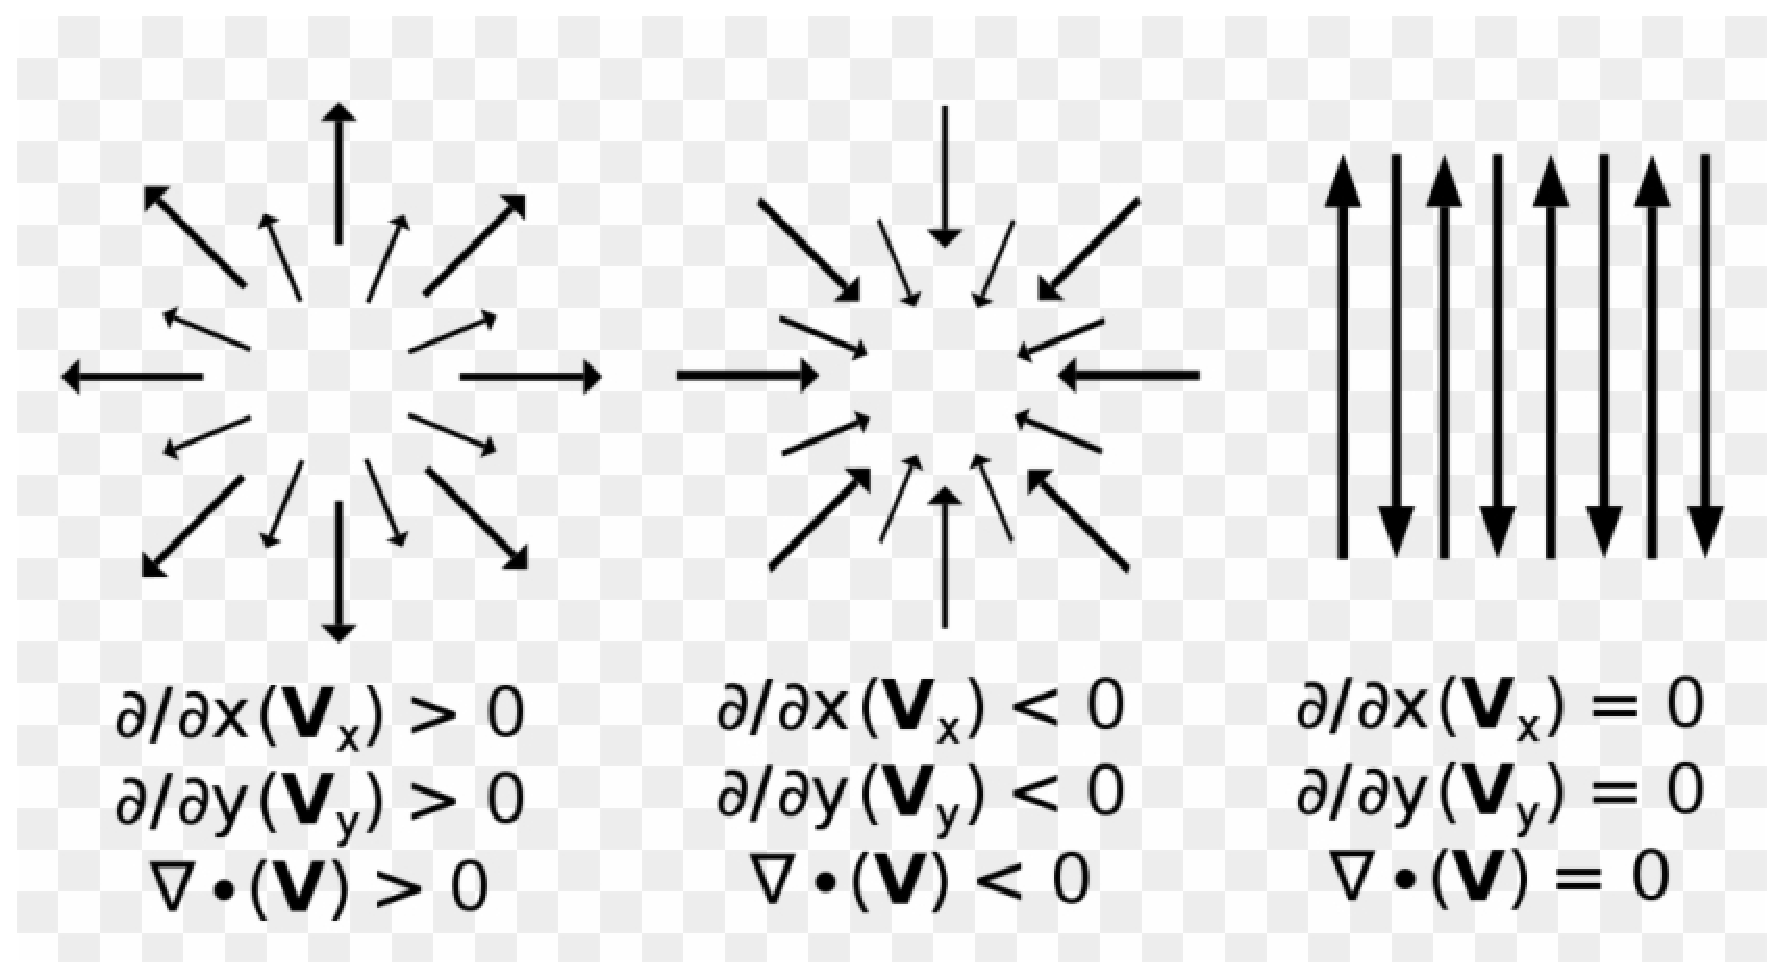
\includegraphics[width=1\textwidth]{maxwell_eq.eps}
  		\caption{Applications of Maxwell's equation}
		\label{fig:fig1}
	\end{center}
\end{figure}



\subsection{Importance of Maxwell's Equations}
Equation \ref{eq:gauss_ele}, also known as Gauss’ Law, is stating that the divergence of the electric field is equal to the charge density inside of a closed surface of interest, multiplied by a constant. The divergence is how much the electric field “spreads out” from a given point. If there is more charge inside, the divergence is greater. If it’s zero, the divergence is zero \cite{Baillet200114}.
\\
\\
What this equation \ref{eq:gauss_mag} is saying is that the curl of the electric field is equal to the negative of the change in the magnetic field in time. In other words, if the magnetic field isn’t changing, electric field lines are straight. If it is changing, the electric field “swirls” appropriately, depending on if the field is increasing or decreasing. A changing magnetic field can induce an electric field! (i.e. Faraday induction). The negative sign is called Lenz’s law.
\\
\\
There are no magnetic monopoles (equation \ref{eq:faraday}). The divergence of B is always zero. As such, there is no “sink” or “source” for B - the field lines have no beginning and no end. There is no source for them like there is for an electric field (i.e. an electric monopole). All magnetic “charge” is found in a dipole, with a North and a South.
\\
\\
The curl of B, or the “swirliness of B” is equal to the Current Density (the amount of current per unit volume) plus any change in the electric field (equation \ref{eq:ampere}). This second part is often called the “displacement current, since it helps with dealing with capacitors \cite{Yee1966302}.
\\
\\
Figure \ref{fig:fig1} is showing different situation of Maxwell equation.






\newpage
\bibliography{reference}
\bibliographystyle{plain}

\end{document}
